\documentclass{article}
\usepackage[margin=24mm]{geometry}
\usepackage{tikz}
\title{Unattended joint quadratic search on Amaterasu}
\date{Created-at: 2026-10-29 19:21 CET}
\begin{document}\maketitle
\paragraph{Goal.} Launch a bounded detached search for a cheaper simultaneous
GF64 norm and inverse-phase coefficient map. The starting factorization has
45 AND products. A reduction to39 could cross the current contextual threshold
at Q889. No improvement is assumed. User explicitly requested unattended native
execution on Amaterasu; no Kaggle upload or incumbent overwrite is authorized.
\paragraph{Ownership.} Quantum owns the degree-two factorization heuristic and
native lowering. It consumes the existing source-bound Hermite recipe and the
reviewed field tensor. This is coefficient-level proposal search, not a new
canonical IR, matroid solver or a replacement for Core/Graph. No provider or
dependency edits. Existing Graph/P-graph evidence remains as before.
\paragraph{Algorithm and proof.} State is at most64 products of two24-bit
linear forms with12-bit output vectors, plus24 linear output vectors. Exact
GF2 tensor flips sharing an input or output factor preserve the polynomial.
Merge identical products, remove zero terms, and turn squares into linear
terms. Check all301 zero/single/pair input points: for degree at most two this
certifies every coefficient over the whole24-input domain. Restart walks from
the best state; stop at target, step limit or wall budget. No optimum claim.
\paragraph{Admission.} Derive the baseline using native GF64 arithmetic and
check it independently. The existing Hermite phase adapter optionally emits
the certified joint map, retaining the same measurement cleanup. Startup and
each improved factorization require phase and cross-paired jet checks. A
contextually promising candidate may receive a complete build and102400-shot
official verification using the fixed salt. Save results; never replace the
accepted883-qubit artifact automatically.
\paragraph{Files.} Add native joint\_search.py and focused tests; extend
hermite.py only at its joint quadratic lowering point. Add a thin detached
launch tool and this plan. Generated launch/provenance snapshots go under
reports; live logs/checkpoints live in the existing remote output directory.
Protected items and new dependencies: none.
\paragraph{Budgets and ETA.} Preparation approximately20--30min. Search at
most7200s/50000000steps, checkpoint every60s and on improvement; reserve a
further1200s for optional complete build/verification. One CPU,12GiB hard and
10000MiB sampled process-tree limit,9000s total guard. Native memory availability
was19GiB and disk317GiB. The ordinary search is small; full circuits need several
GiB. Check available memory before the full stage. Failures produce a durable
failed status rather than an accepted candidate.
\paragraph{Execution.} Use the existing pinned Python image and read-only
runtime/public-source mounts. Pass current code in compressed in-memory input;
no remote source checkout, WSL or duplicate build target. Verify container and
checkpoint state before reporting launch. SSH/client disconnection must not stop
the Docker job. Preserve an exact source/config identity and named stop command.
\paragraph{Validation and rollback.} Unit tests cover flip invariance,
normalization, coefficient checks and tampering. Native smoke precedes the long
launch. Reject failed phase/workspace checks. Stop only the owned named container;
retain checkpoints and logs. Network settings and other services stay unchanged.
\begin{center}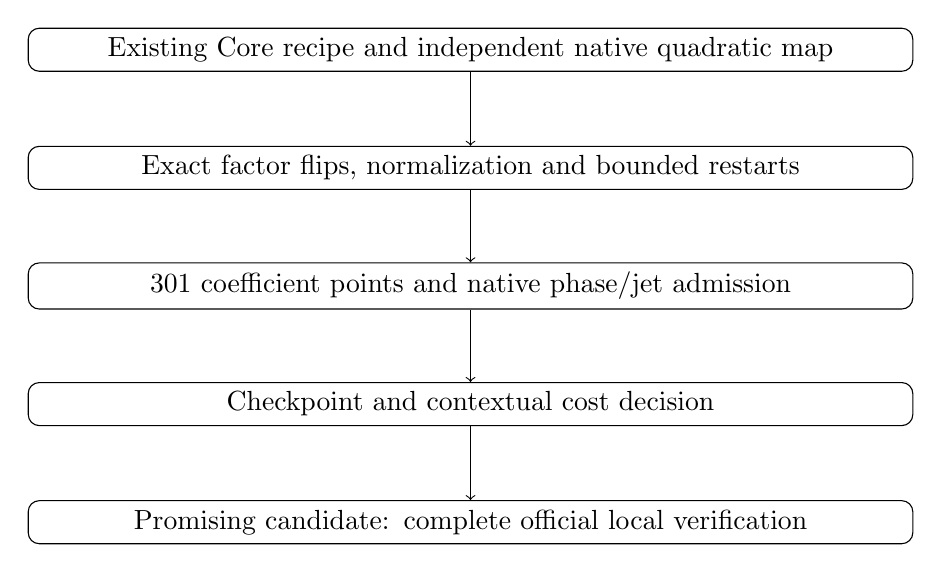
\begin{tikzpicture}[every node/.style={draw,rounded corners,align=center,text width=11cm},node distance=15mm]
\node (a) {Existing Core recipe and independent native quadratic map};
\node (b) [below of=a] {Exact factor flips, normalization and bounded restarts};
\node (c) [below of=b] {301 coefficient points and native phase/jet admission};
\node (d) [below of=c] {Checkpoint and contextual cost decision};
\node (e) [below of=d] {Promising candidate: complete official local verification};
\draw[->] (a)--(b);\draw[->] (b)--(c);\draw[->] (c)--(d);\draw[->] (d)--(e);
\end{tikzpicture}
\end{center}
\end{document}
